\section{Object-Orientierung}
\subsection{Objekte zur Laufzeit}
\begin{itemize}
    \item Ablage erzeugter Objekte auf Heap
    \item Heap: Linearer Adressraum
\end{itemize}
\textbf{Wiso werden Objekte nicht auf dem Stack augelegt?}
\begin{itemize}
    \item Sie würden Methoden-Ende nicht überleben, sondern mit Activation Frame zerstört werden.
\end{itemize}
\textbf{Objekt Lebenszeit}
\begin{itemize}
    \item Nicht an Methodeninkarnatiion gebunden
\end{itemize}

\subsubsection{Deallokation}
\begin{itemize}
    \item Keine Hierarchie unter Objekten
    \item Keine hierarchische Lebensdauer
    \item Deallokation verursacht Lücken
\end{itemize}

\subsection{Unmanaged Memory in Java}
\begin{itemize}
    \item Speicher über Java Native Access allozieren
    \item Raw Heap kann keine Java Referenzen speichern! Stattdessen Map verwenden (\textit{HashMap\textless Long, Object\textgreater})
\end{itemize}
\begin{lstlisting}
import com.sun.jna.Memory;

Memory heap = new Memory(HEAP_SIZE);

long value = heap.getLong(address); // 64-bit lesen, address = offset im Heap
// ... 
heap.setLong(address, value);
\end{lstlisting}

\subsubsection{Objektblock im Raw Heap}
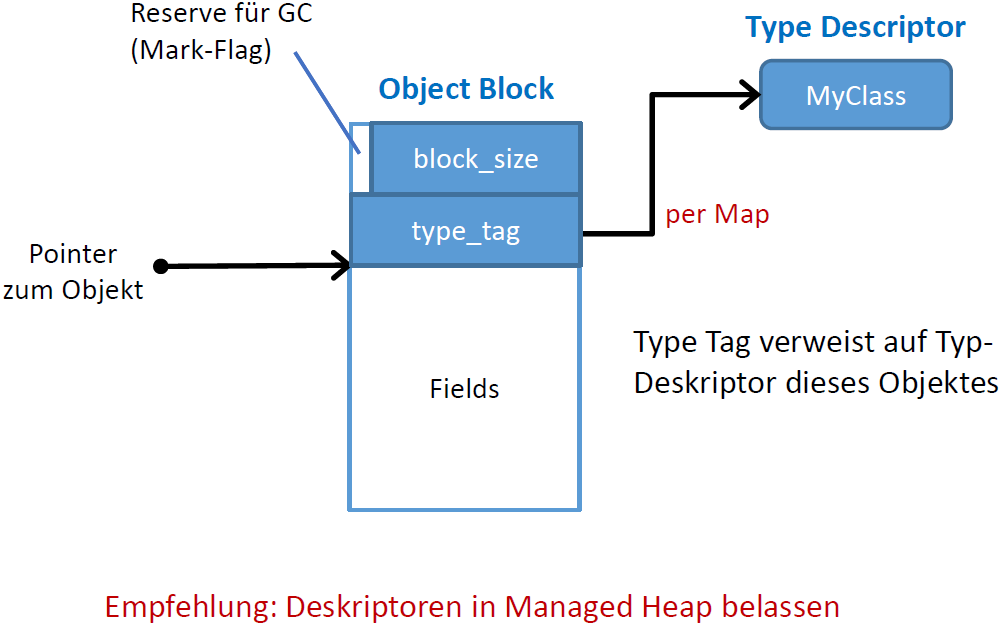
\includegraphics[width=0.5\linewidth]{raw_heap.png}
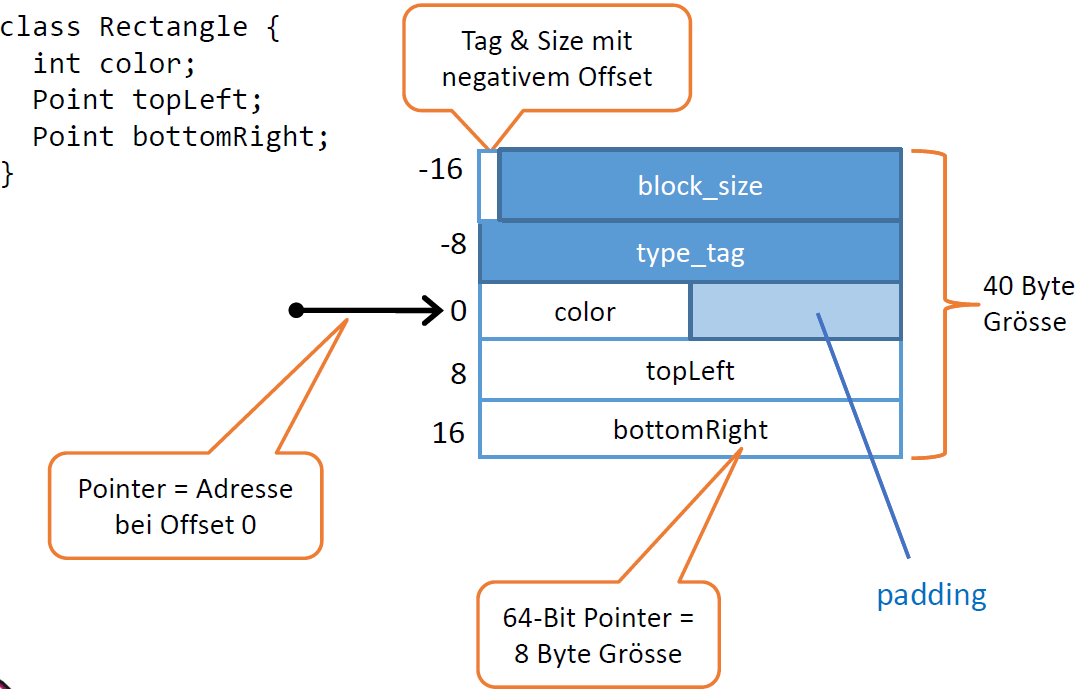
\includegraphics[width=0.5\linewidth]{raw_heap2.png}

\subsubsection{Array Block}
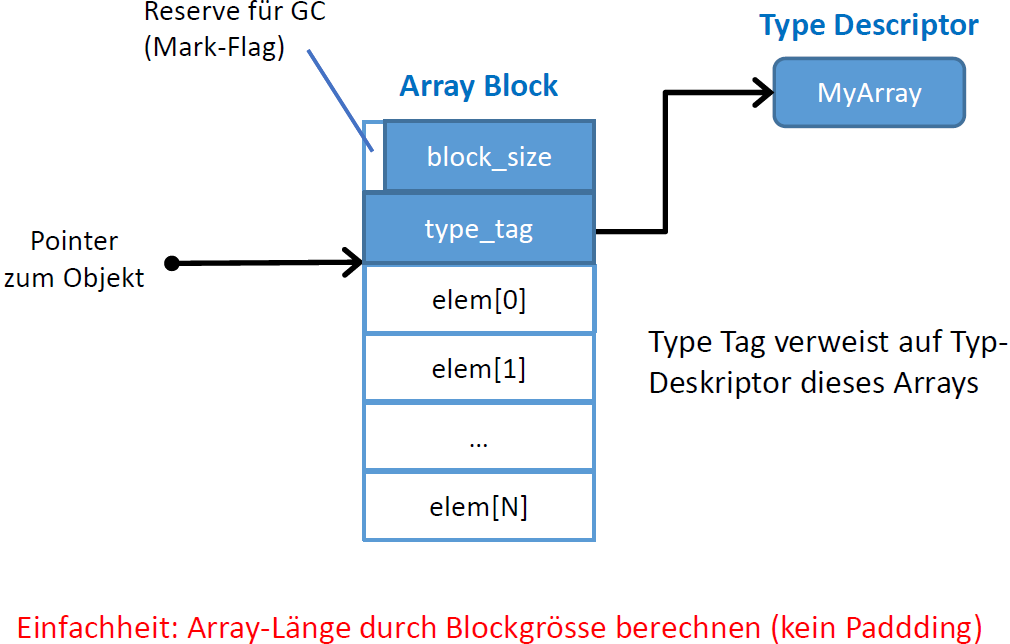
\includegraphics[width=0.5\linewidth]{array_block.png}

\subsubsection{Heap-Allokation}
\begin{lstlisting}
Pointer allocate(int size, TypeDescriptor type) {
    int blockSize = size + 16; // Mit Header
    if(freePointer + blockSize > limit) {
        throw new VMException("Out of Memory");
    }
    long address = freePointer;
    freePointer += blockSize;
    heap.setLong(address, blockSize);
    setTypeDescriptor(type, address);
    address += 16;
    return new Pointer(address);
}

Pointer allocateObject(ClassDescriptor type) {
    int size = type.getAllFields().length * 8; // Einfaches Layout 
    return allocate(size, type);
}

Pointer allocateArraay(ArrayDescriptor type, int length) {
    int size = length * 8;
    return allocate(size, type);
}
\end{lstlisting}